% include the figures path relative to the master file
\graphicspath{ {./content/method/figures/visual_cues/}{./content/method/figures/}}

\section{Description of the segmentation methodology} 

Optimization methodologies offer a standardized manner to approach segmentation by minimizing an application-driven cost function~\cite{cremers2007review}.
Figure~\ref{fig:method} illustrates a generic representation of the segmentation strategy here adopted to delineate breast tissues or lesions in \ac{us} images. 
The overall segmentation can be seen as a three-steps strategy: 
(1) a mapping of the image into a discrete set of elements $\mathcal{S}$, 
(2) the optimization stage which is formulated as a \emph{metric labelling} problem, 
and (3) a re-mapping the labels obtained from the previous stage to produce the final delineation. 

\begin{figure}[htpb]
  \centering
  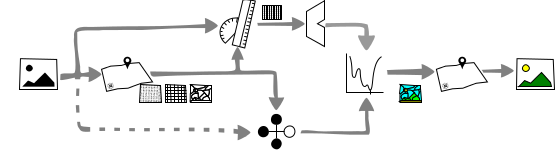
\includegraphics[width=0.9\linewidth]{method}
  \caption{Conceptual block representation of the segmentation methodology}
  \label{fig:method}
\end{figure}


In order to formulate the segmentation like a metric labelling problem, the image is conceived as a discrete set of elements $\mathcal{S}$ that need to be labelled using a label $l$ from the labelling set $\mathcal{L}$.
Let $\mathcal{W}$ be all the possible labelling configurations of the set $\mathcal{S}$, given $\mathcal{L}$.
Let $U(\cdot)$ be a cost function encoding the goodness of the labelling configuration $\omega \in \mathcal{W}$ based on the appearance of the elements in $\mathcal{S}$, their inner relation and some designing constraints.
Then, the desired segmentation $\hat{\omega}$ corresponds to the labelling configuration that minimizes this cost function, as described in Eq.\,\eqref{eq:costMin}.

\begin{equation}
\hat{\omega} = \arg \min_{\substack{\omega}} \,U(\omega)
\label{eq:costMin}
\end{equation}

It is worth to mention here that not all the minimization strategies are applicable or adequate to find $\hat{\omega}$.
The convenience of a particular minimization strategy is determined by the nature of $U(\cdot)$ and $\mathcal{W}$ (see Sect.\,\ref{sec:method:min}).

This goodness measure $U(\cdot)$ must be defined to take into account the appearance of the target region, its relation with other regions and other designing constraints.
Equation~\eqref{eq:labelingeq} describes this cost function as the combination of two independent costs that need to be simultaneously minimized as a whole.

\begin{equation}
  U(\omega) = \sum_{s\in \mathcal{S}} D_s(\omega_s) + \sum_{s \in \mathcal{S}}\sum_{r \in \mathcal{N}_{s}} V_{s,r}(\omega_s,\omega_r)
  \label{eq:labelingeq}
\end{equation}

Where, the left hand side of the expression integrates the so-called \emph{data} term, while the right hand side integrates the \emph{pairwise} term, which is also referred as the \emph{smoothing} term.
Both terms are shaped by $\mathcal{S}$ and evaluated in the labelling space $\mathcal{W}$.
Figure~\ref{fig:methodterms} uses the problem of delineating the tissues present in a \ac{bus} image to represent the working principles of the data and pairwise terms in Eq.\,\eqref{eq:labelingeq}.
In general, $\mathcal{S}$ can be any discrete set representing the image (i.e.\, pixels, overlapping or non overlapping windows, super-pixels, etc.). 
Figure~\ref{fig:methodTerms:problem} illustrates one such representation $\mathcal{S}$, applied to a \ac{bus} image example using super-pixels. The super-pixels are coloured according to the image's \ac{gt}.


\begin{figure}
    \centering
    \begin{subfigure}[b]{0.19\textwidth}
        \centering
        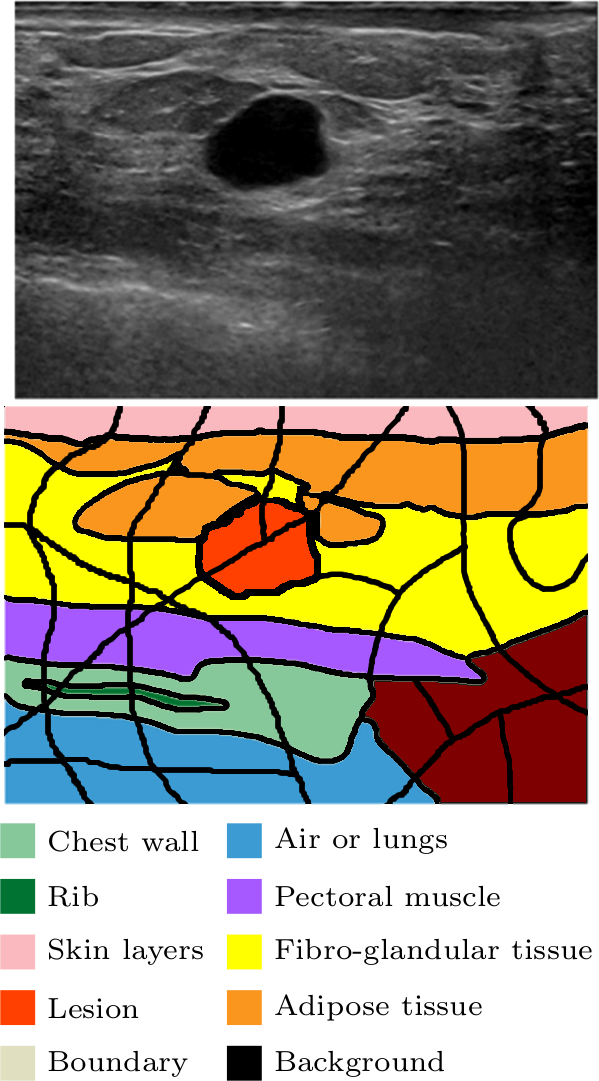
\includegraphics[width=\textwidth]{problem}
        %\caption{{\small Problem definition}}    
        \label{fig:methodTerms:problem}
    \end{subfigure}
    \hfill
    \begin{subfigure}[b]{0.39\textwidth}  
        \centering 
        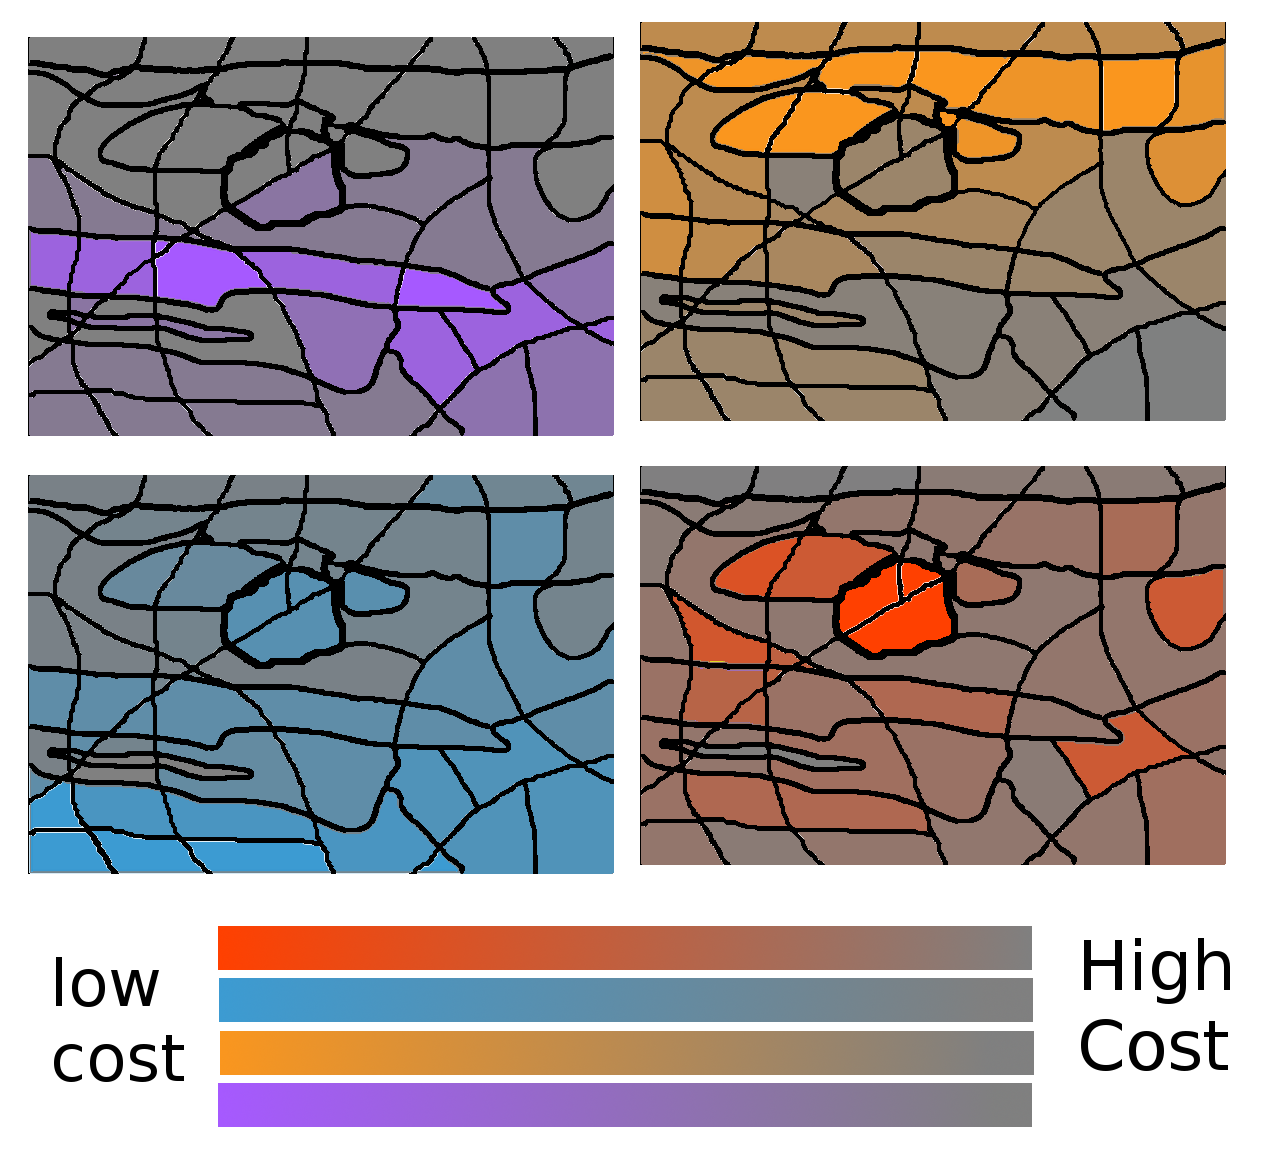
\includegraphics[width=\textwidth]{data}
        %\caption[]% {{\small Data term}}    
        \label{fig:methodTerms:data}
    \end{subfigure}
    \hfill
    \begin{subfigure}[b]{0.39\textwidth}   
        \centering 
        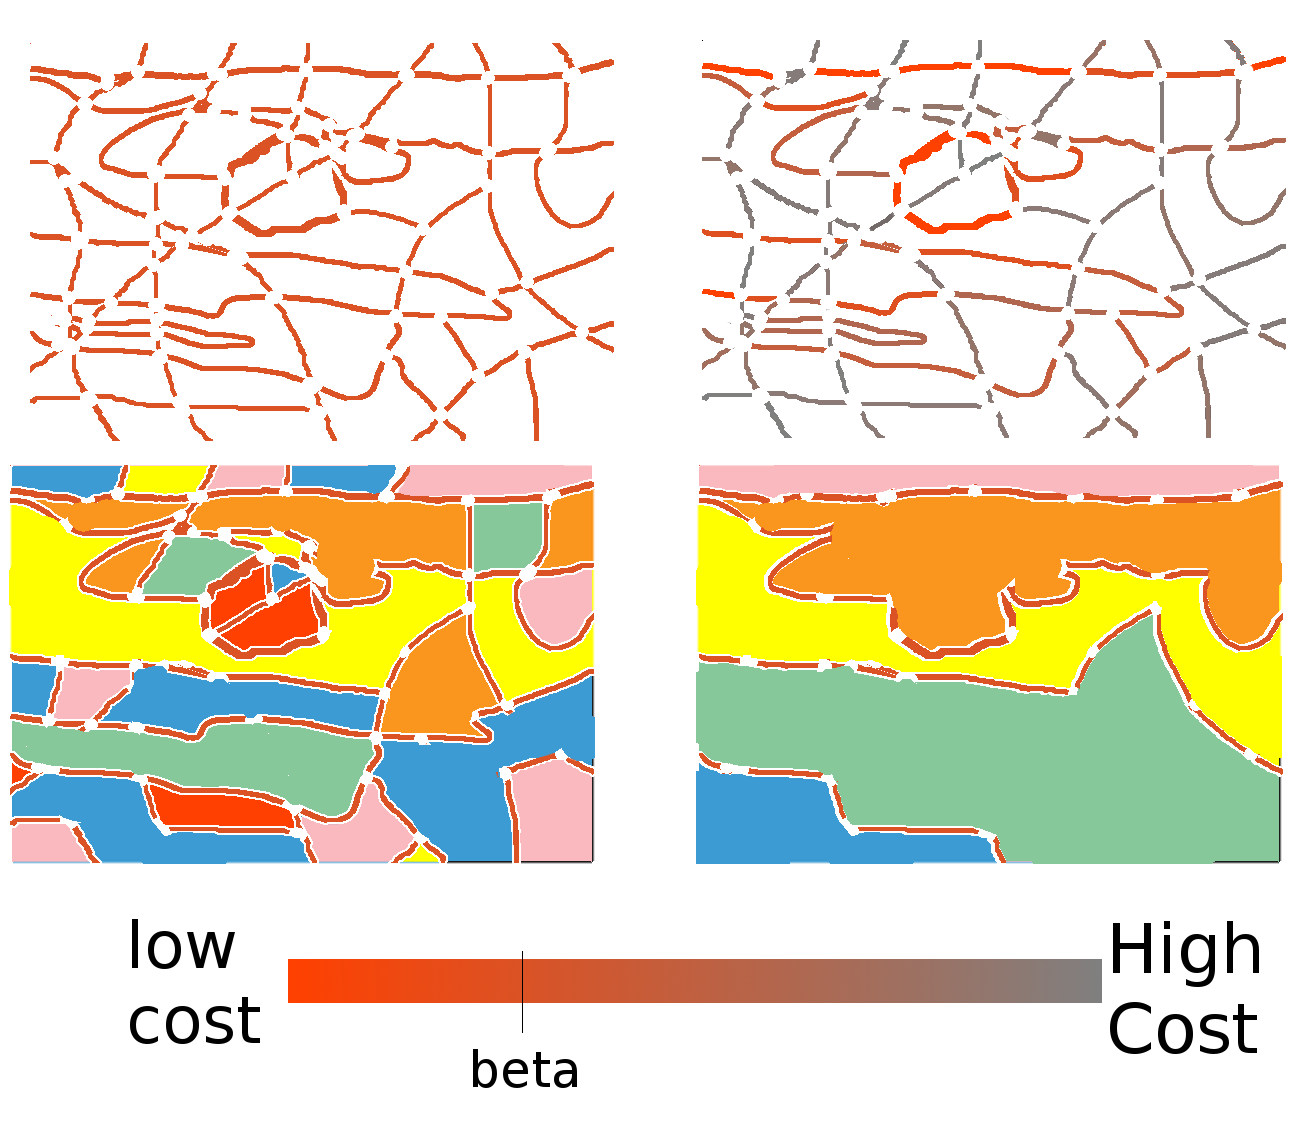
\includegraphics[width=\textwidth]{smooth} 
        %\caption[]% {{\small Pairwise term }}
        \label{fig:methodTerms:boundary}
    \end{subfigure}
    \caption {\small Methodology: (a) Problem definition, (b) Data term, (c) Pairwise term.} 
    \label{fig:methodterms}
\end{figure}

{\color{red}In our quest to optimize the cost function $U(\cdot)$, it is required to define a representation for the set $\mathcal{S}$, a data term $D(\cdot)$, a pairwise term $V(\cdot)$, and a proper minimization methodology.}

\subsection{The data term} \label{sec:method:dataTerm}

Given a label configuration $\omega \in \mathcal{W}$, the data term penalizes the labelling of a particular image element or site ($\omega_s = l$) based on the data associated to $s$.
In this manner, $D_s(\omega_s=l_\cmark) << D_s(\omega_s=l_\xmark)$.
Figure~\ref{fig:methodTerms:data} illustrates the data cost associated to some arbitrary labelling configurations to clarify the desired effect (or behaviour) of this data term (Fig.\,\ref{fig:methodTerms:problem} shows the \ac{gt} of each site $s$).

Designing an obscure heuristic to comply with the desired behaviour of $D(\cdot)$ out of the box, is rather a complicated task.
Therefore, an easier and cleaner approach is to take advantage of \ac{ml} techniques to design this data cost in a systematic manner based on a training stage. 
The idea is to generate a data model for each label (or class) in $\mathcal{L}$ from training samples, and let $D(\cdot)$ be a distance or goodness measure reflecting the likelihood for $s$ to belong to class $l$.
\ac{ml} offers a systematic but flexible approach to customize $D(\cdot)$.
Different features to represent the data, custom construction of the data models by using different classifiers, training techniques or including arbitrary constraints; can be used to achieve the desired data term without changing the overall scheme. 

{\color{red} Defining the data term $D(\cdot)$ with the help of \ac{ml} follows a systematic process. For each site $s \in \mathcal{S}$, features describing $s$ have to be detected. Then, different optional steps can be applied to this set of feature: (i) features normalization, (ii) features selection or (iii) features extraction. Finally, the data term $D(.)$ is encoded based on \ac{ml} classifiers, the features and a training step. This representation is in fact depicted in the upper row in Fig.\,\ref{fig:method}.}

\subsection{The pairwise term} \label{sec:method:mrfTerm}
 
The pairwise term represents the cost associated to $\omega_s$ taking into account the labels of its neighbour sites, $\omega_r$, $r \in \mathcal{N}_{s}$. 
This term models a \ac{mrf} or a \ac{crf}.
The typical form of this term, given in Eq.\,\eqref{eq:smoothing}, is called homogenization which acts as a regularization factor favouring configurations that have a coherent labelling.

\begin{equation}
V_{s,r}(\omega_s,\omega_r) = 
\begin{cases}
    \beta, & \text{if } \omega_s \ne \omega_r\\
    0,              & \text{otherwise}
\end{cases}
\label{eq:smoothing}
\end{equation}

Figure~\ref{fig:methodTerms:boundary} offers a visual interpretation of this cost.
The more fragmented is the segmentation $\omega$, the higher the overall pairwise term; since every boundary brings a penalization $\beta$ to the total cost $U(\omega)$.
In this manner the regularization term can be seen as a post-processing or denoising stage since that some sites will flip their labelling if the cost of fragmenting the regions is larger than the cost of adopting their neighbour's label.

% Review %contribute have different or variable costs (see \cref{fig:methodTerms:boundary}) are also possible by taking into account not only relations in $\mathcal{S}$ of but also image information (see \cref{fig:method}). 
%Further details can be found in \cref{sec:smoothing}.

\subsection{Searching the best labelling configuration} \label{sec:method:min}
Once defined $U(\omega)$ so that the cost for a particular labelling configuration $\omega$ can be computed, the problem of finding $\hat{\omega}$ corresponding to the global minimum of the space $\mathcal{W}$ of all possible labelling configurations needs to be faced. 
%
%%This problem falls into the category of \textbf{NP-hard} problems. 
%% Good % The dimension of the solution space can be expressed as $||\mathcal{W}|| = ||\mathcal{L}||^{||\mathcal{S}||}$. 
%% Good % This means that in order to perform an exhaustive search for a toy example of $20$ sites and two possible labels, the cost function needs to be calculated way more than a million times. 
%%Moreover, due to limitations in building $U(\cdot)$ such as noise, training policies, etc. there are no guarantees that the global minimum $\hat{\omega}$ corresponds to the true labelling.
%
%%Nevertheless, there is a large body of literature proposing methodologies to find suboptimal solutions to the problem trading-off between time of convergence and accuracy of the solution reached.
%%Szeliski et al.~\cite{szeliski2008comparative} conducted an exhaustive review in terms of solution quality and runtime of the most common energy minimization algorithms used in \ac{cv}, such as \ac{icm}, \ac{sa} or \ac{gc}.
%
%%The minimization strategy used for this work is \ac{gc}. 
%%This technique was initially introduced to solve \ac{cv} applications by Boykov et al.~\cite{boykov2001fast}.
%%Soon after its introduction, it becomes the minimization technique of choice for \ac{cv} problems.

% Good % \subsection{Similitude with other optimization techniques}
% Good % \todo{needs reworking}
% Good % It is worth to mention here, that this pairwise term links this segmentation strategy to the family of segmentation methodologies based on optimization using \ac{acm}, such as levelsets.
% Good % On its basic form, the family of \ac{acm} segmentation defines some forces to be applied to an initial contour and this contour evolves by minimizing its length while constrained by the forces properly designed for the task in hand.

%%% Local Variables: 
%%% mode: latex
%%% TeX-master: "../../master.tex"
